As an alternative to Google Play, started its own application store in October 2010 with the goal to generate profits from selling apps on Android as well \cite{amazonBeta}.
It was opened to the public on the 03/22/2011 for Android and Fire tablets \cite{amazonRelease}.
The store comes with its own DRM since the Google LVL only works with the Google Play Store.
The developer can chose whether it should be enabled in the developer console  in their developer console.
When reengineering the \gls{apk} the added code can be found in a package called \textit{Kiwi} as seen in figure~\ref{fig:amazonFolder}. \cite{amazonDeveloper}
\begin{figure}[h]
    \centering
    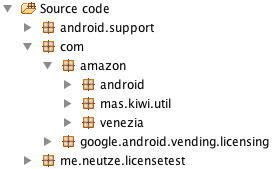
\includegraphics[width=0.3\textwidth]{data/amazonFolder.png}
    \caption{Amazon library structure in decompiled application}
    \label{fig:amazonFolder}
\end{figure}
